\documentclass[tikz,border=1pt]{standalone}
\begin{document}
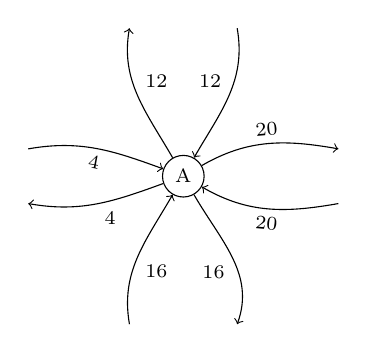
\begin{tikzpicture}[auto,scale=2]\scriptsize
	\node[circle,draw] (N) {A};
	\draw[->] (N) to[out=120,in=-100]	node[swap]			{12}  +(110:1);
	\draw[<-] (N) to[out=60,in=-80]		node[]				{12} +( 70:1);
	\draw[<-] (N) to[out=160,in=10]		node[swap,sloped]		{4}  +(170:1);
	\draw[->] (N) to[out=200,in=-10]	node[]				{4}  +(190:1);
	\draw[<-] (N) to[out=-120,in=100]	node[]				{16}  +(250:1);
	\draw[->] (N) to[out=-60,in=70]		node[swap]			{16} +(-70:1);
	\draw[->] (N) to[out=30,in=170]		node[sloped]			{20} +( 10:1);
	\draw[<-] (N) to[out=-30,in=190]	node[sloped,swap]		{20} +(-10:1);
\end{tikzpicture}
\end{document}
